\section{Our Dataset}\label{paperA:sec:our-dataset}

\begin{wrapfigure}{r}{0.44\textwidth}
	\centering
	%\hspace{-6mm}
	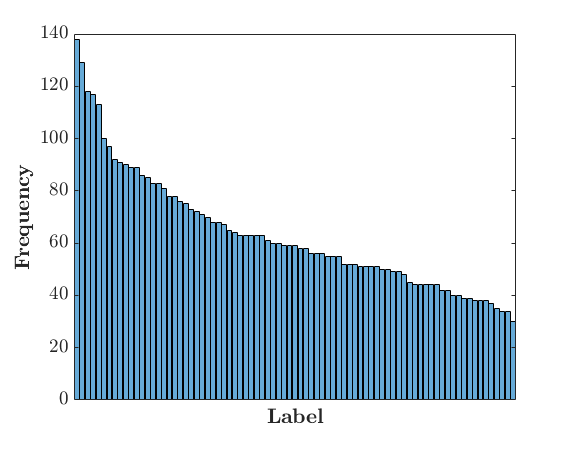
\includegraphics[width=0.44\textwidth, height=0.23\textwidth]{PaperA/figures/hist1_latex_bf14.png}
	\vspace{-6mm}
	\captionsetup{width=.88\linewidth}
	%\hspace{-6mm}
	\caption{Histogram over the number of images in each class in the dataset.}
	\vspace{-2mm}
	\label{fig:hist}
\end{wrapfigure}
We have collected images from fruit and vegetable sections and refrigerated sections with dairy and juice products in 18 different grocery stores. The dataset consists of 5125 images from 81 fine-grained classes, where the number of images in each class range from 30 to 138. Figure \ref{fig:hist} displays a histogram over the number of images per class. As illustrated in Figure \ref{fig:examples}, the class structure is hierarchical, and there are 46 coarse-grained classes. Figure \ref{fig:dataset-figure} shows examples of the collected natural images. For each fine-grained class, we have downloaded an iconic image of the item and also a product description including origin country, an appreciated weight and nutrient values of the item from a grocery store website. Some examples of downloaded iconic images can be seen in Figure \ref{fig:clean-image-figure}. 

Our aim has been to collect the natural images under the same condition as they would be as part of an assistive application on a mobile phone. All images have been taken with a 16-megapixel Android smartphone camera from different distances and angles. Occasionally, the images include other items in the background or even items that have been misplaced in the wrong shelf along with the targeted item. It is important that image classifiers that are used for assisting devices are capable of performing well with such noise since these are typical settings in a grocery store environments. The lighting conditions in the images can also vary depending on where the items are located in the store. 
Sometimes the images are taken while the photographer is holding the item in the hand. This is often the case for refrigerated products since these containers are usually stacked compactly in the refrigerators. For these images, we have consciously varied the position of the object, such that the item is not always centered in the image or present in its entirety. 

We also split the data into a training set and test set based on the application need. Since the images have been taken in several different stores at specific days and time stamps, 
parts of the data will have similar lighting conditions and backgrounds for each photo occasion. To remove any such biasing correlations, all images of a certain class taken at a certain store are assigned to either the test set or training set. Moreover, we balance the class sizes to as large extent as possible in both the training and test set. After the partitioning, the training and test set contains 2640 and 2485 images respectively. Predefining a training and test set also makes it easier for other users to compare their results to the evaluations in this paper.

The task is to classify natural images using mobile devices to aid visually impaired people. The additional information such as the hierarchical structure of the class labels, iconic images, and product descriptions can be used to improve the performance of the computer vision system. Every class label is associated with a product description. Thus, the product description itself can be part of the output for visually impaired persons as they may not be able to read what is printed on a carton box or a label tag on a fruit bin in the store.

%Collecting and labeling real-world data is a time-costly procedure. 
%Therefore, we propose that the natural images can be combined with additional information of the target object in the form of text and iconic images.
The dataset is intended for research purposes and we are open to contributions with more images and new suitable classes. Our dataset is available at \url{https://github.com/marcusklasson/GroceryStoreDataset}. Detailed instructions on how to contribute to the dataset can be found on our dataset webpage.


\begin{comment}
\begin{figure}[t]
\centering
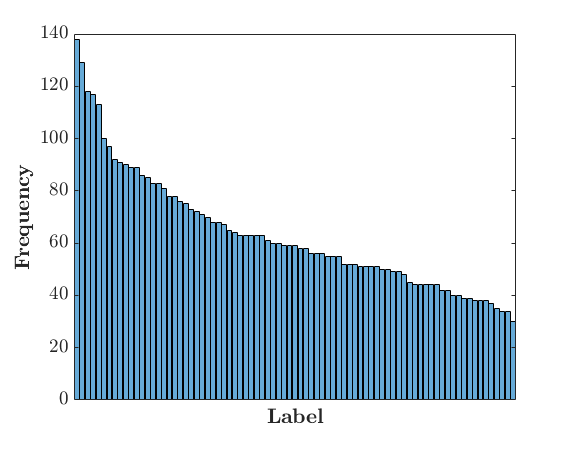
\includegraphics[width=\columnwidth,height=0.20\paperheight]{PaperA/figures/hist1_latex_bf14.png}
\caption{Histogram over the number of images in each class in the dataset.}
\label{fig:hist}
\end{figure}
\end{comment}

